\documentclass[a4paper]{article}

\usepackage{listings}
\usepackage{graphicx}
\usepackage{tabularx}
\usepackage{tikzsymbols}
\usepackage{hyperref}
\usepackage{amsmath}
\usepackage{amssymb}

\usepackage[margin=2cm]{geometry}

\usepackage{titlesec}
\titleformat*{\section}{\large\bfseries}

\definecolor{kit-blue}{RGB}{70, 100, 170}
\input{../slides/l00-commands.tex}

\begin{document}
\exhead{2}{2025-05-20}{2024-06-03}

\newcommand{\statetilled}{T}
\newcommand{\statetobetilled}{$+$}
\newcommand{\statenottobetilled}{$-$}

\section{Competition: SDVSTP (8(+8) Points)}

Consider the well-known and industrially relevant \textit{Stardew Valley Soil Tilling Problem} (SDVSTP), which we also talked about (in a slightly simpler form) in the 0th exercise.
\\
We have a $w \times h$ 2D grid $G$ of ``soil'' cells. Each of the $w\cdot h$ cells is in exactly one of the following states: \emph{tilled} (\statetilled), \emph{should be tilled} (\statetobetilled), or \emph{must not be tilled} (\statenottobetilled).
We also define the following five \textit{patterns} (corresponding to five increasing \textit{charging levels} of a hoe):

\begin{figure}[h!]
	\centering
	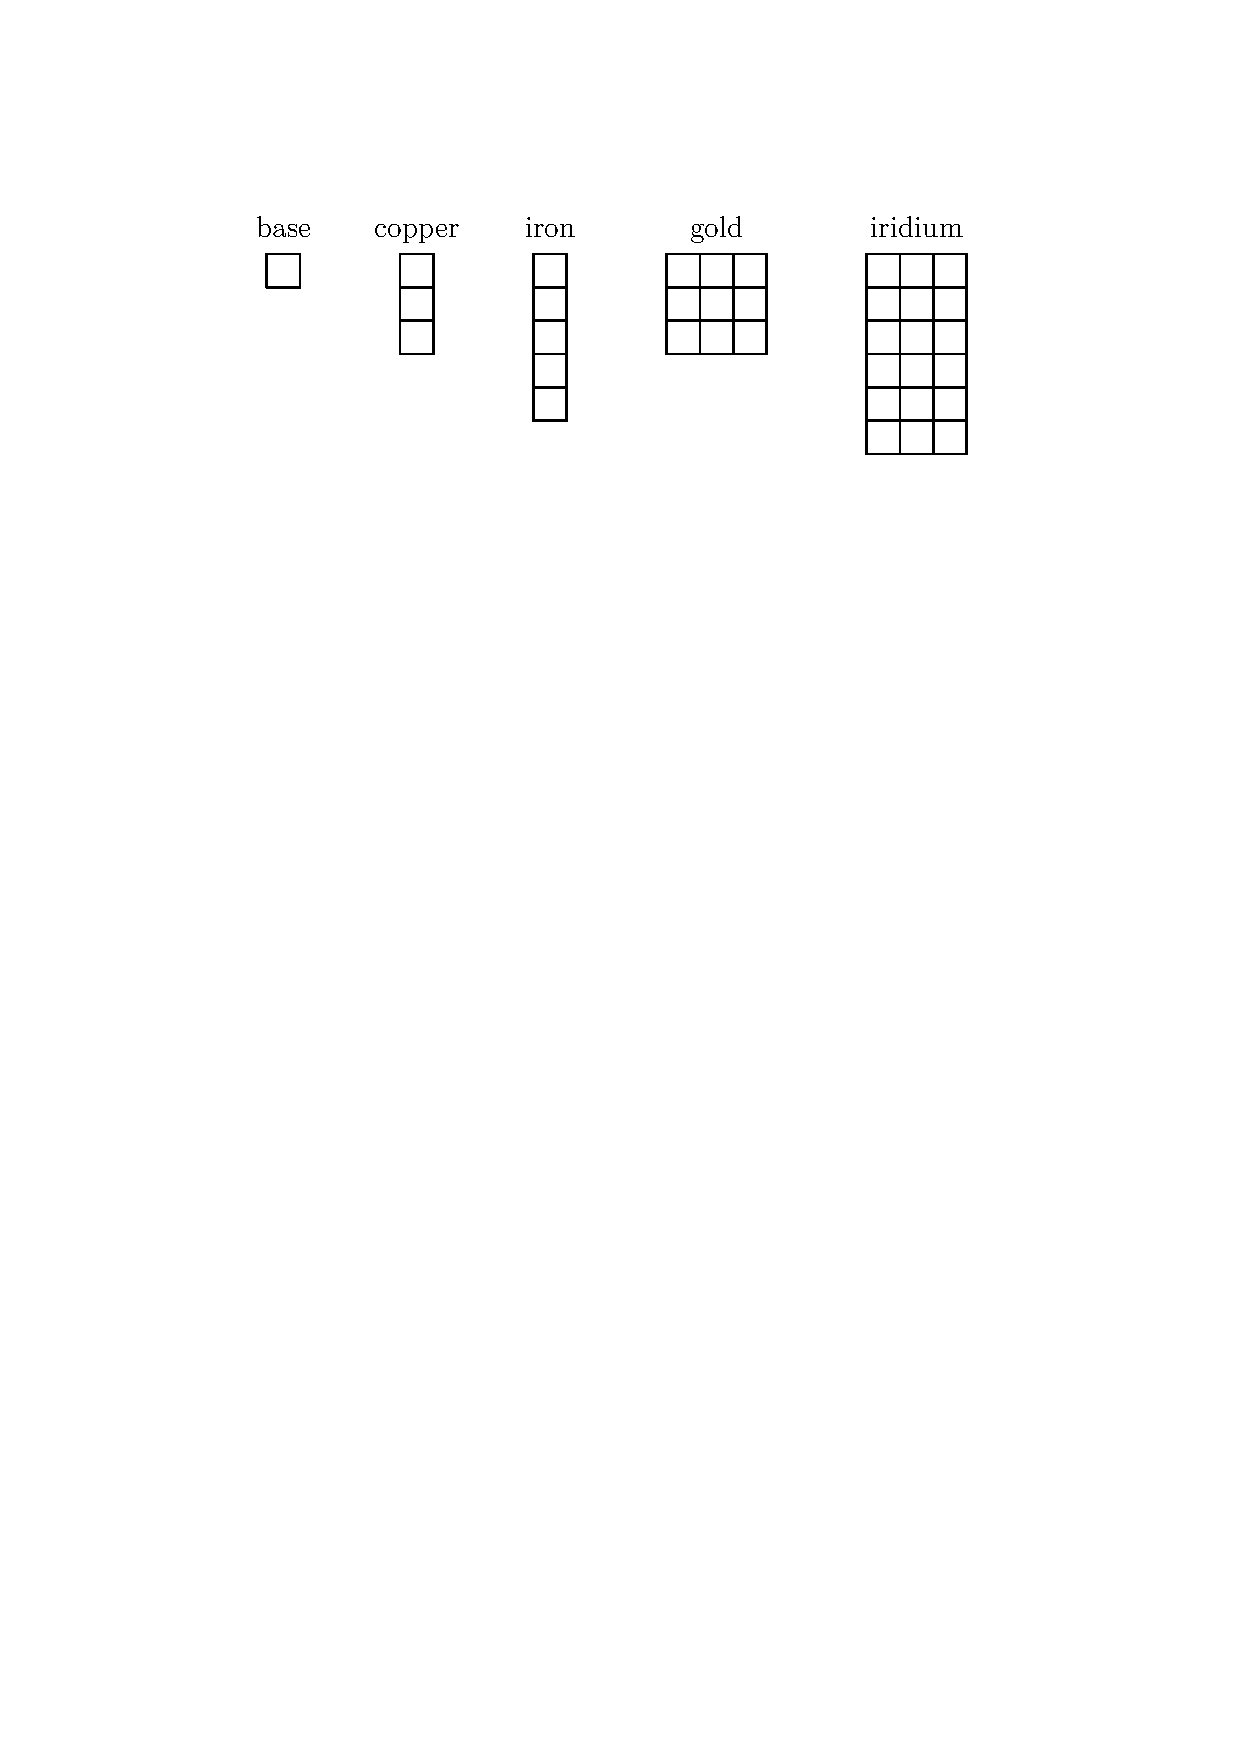
\includegraphics[width=0.475\textwidth]{figures/sdvstp-patterns.pdf}
\end{figure}
\noindent
We further define \emph{action} $a = (p,r,x,y)$ as follows: Rotate the pattern $p \in \{$base, copper, iron, gold, iridium$\}$ by $r \in \{0^\circ, 90^\circ\}$ and then align its \textit{upper left corner} with grid position $(x,y)$.
Then $a$ is \textit{applicable} if the pattern is fully contained within $G$.
Applying $a$ changes all cells in $G$ under the pattern to state \statetilled.

A \textit{solution} for $G$ is a set of applicable actions $A = \{ a_1, a_2, \ldots, a_k \}$ such that applying each action in $A$ transforms $G$ into the grid $G'$ where all cells that were initially in state \statetobetilled{} are in state \statetilled{} and all cells that were initially in state \statenottobetilled{} are still in state \statenottobetilled{}.
The objective is to find a solution that minimizes $k$.

Devise a SAT-based SDVSTP solver.
Your program should take a single argument, the path to an input file in the straight-forward \texttt{.sdvstp} format, structured as in the example in Fig.~\ref{fig:sdv-sol} (left).
The solver should output a line ``\texttt{s SOLUTION k}'', where $k$ is the minimum number of required actions, followed by $k$ lines describing each individual action $(p,r,x,y) \in A$, as in Fig.~\ref{fig:sdv-sol} (center).

\begin{figure}[h!]
	\begin{minipage}{0.33\textwidth}
		\begin{verbatim}
			p sdvstp 8 5
			++++++++
			++++++++
			++T--+++
			+TT--+++
			-------+
			
		\end{verbatim}
	\end{minipage}%
	\begin{minipage}{0.33\textwidth}
		\begin{verbatim}
			s SOLUTION 6
			v gold    0 0 0
			v gold    0 5 1
			v iron   90 3 0
			v copper 90 3 1
			v base    0 0 3
			v base    0 7 4
		\end{verbatim}
	\end{minipage}%
	\begin{minipage}{0.33\textwidth}
		\centering
		\vspace*{2mm}
		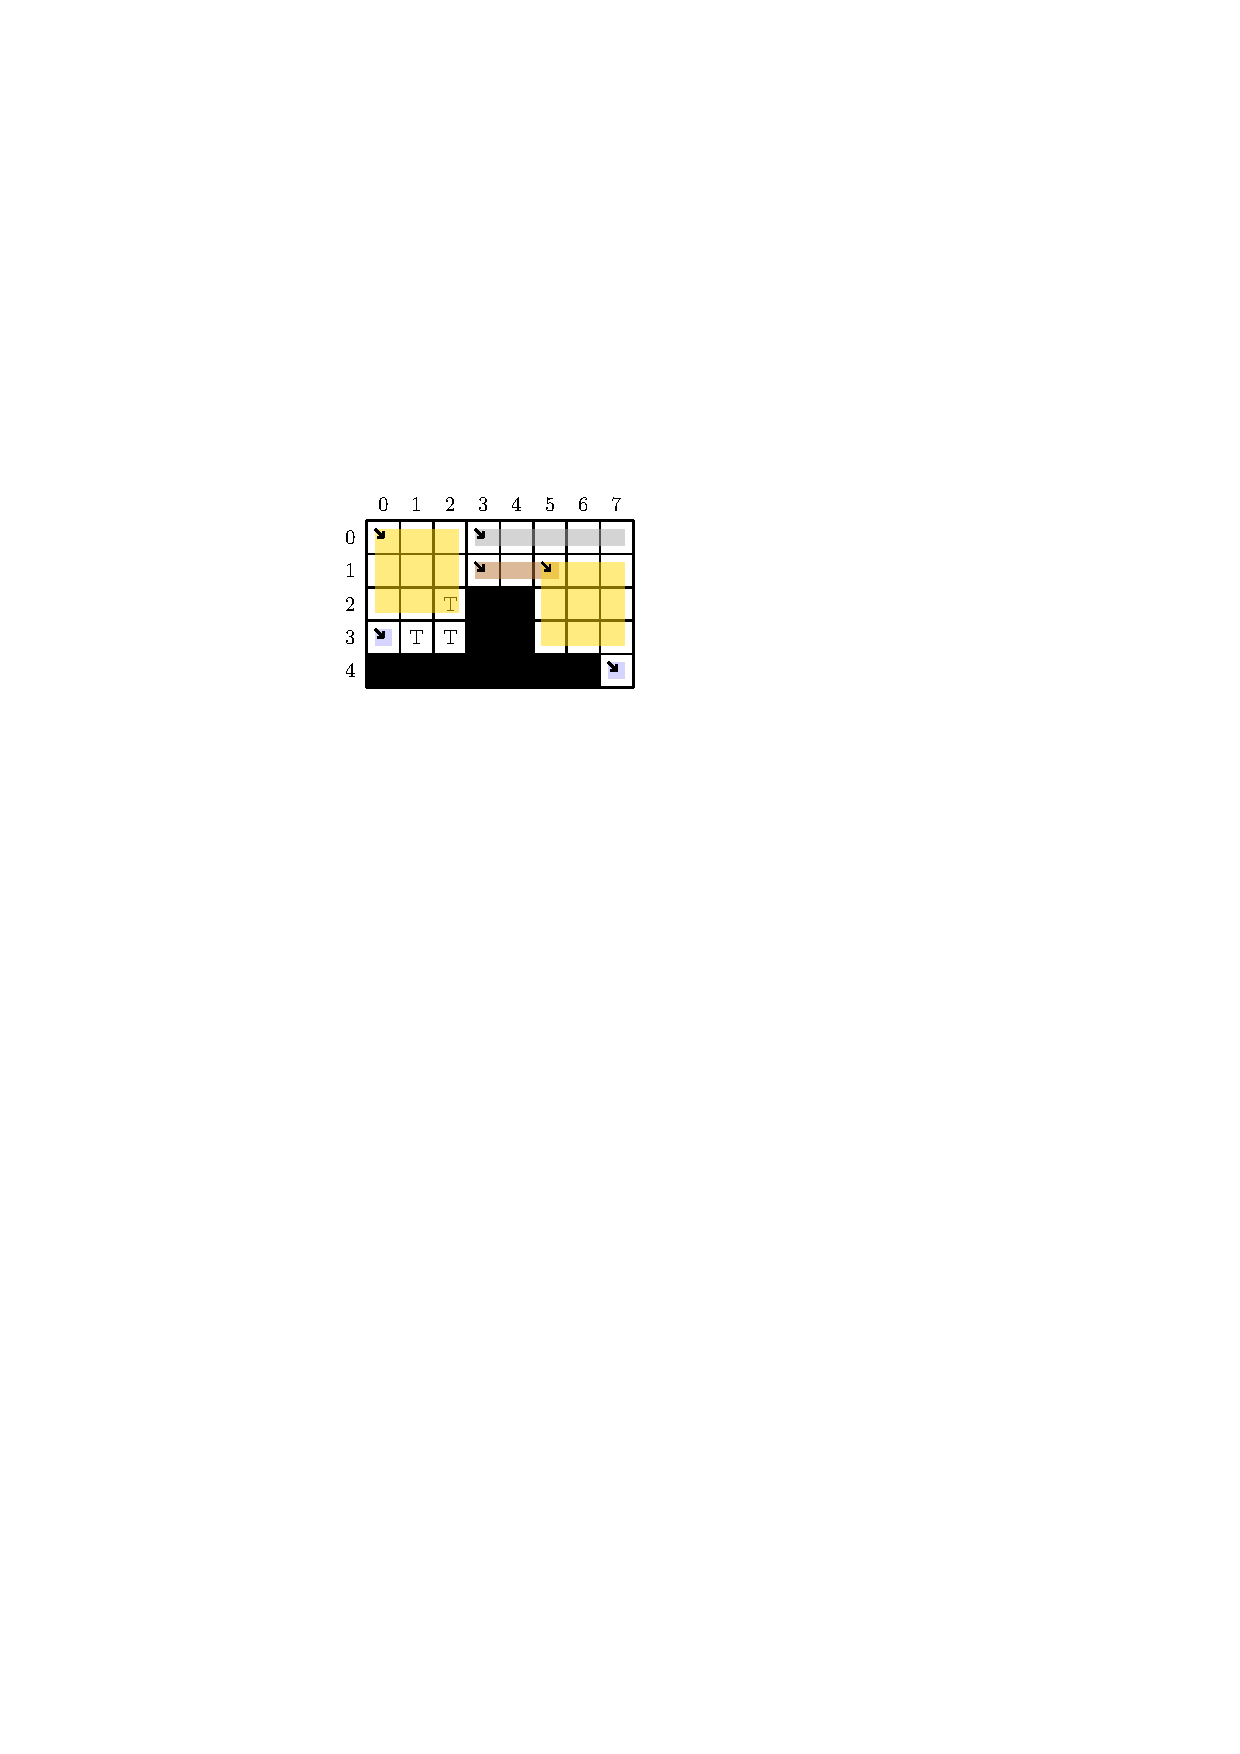
\includegraphics[width=0.8\textwidth]{figures/sdvstp-solution.pdf}\\[2mm]
		~
	\end{minipage}%
	\caption{Left: Example \texttt{.sdvstp} input file specifying an $8\times 5$ grid.
	Center: Possible corresponding output of the solver (columns aligned only for better readability).
	Right: illustration of the grid and the output solution, with the top-left ``anchor point'' of each pattern marked with an arrow.
	}
	\label{fig:sdv-sol}
\end{figure}

You get 8 points for a correct SDVSTP solver that is able to solve easy instances within a few minutes.
The best performing solution is awarded double the points.

\vspace*{3mm}
\noindent
\textbf{Code skeleton:} \url{https://github.com/satlecture/kit2025/blob/main/code/src/sdvstp.cc}

\noindent
\textbf{Some benchmark instances:} \url{https://github.com/satlecture/kit2025/tree/main/exercises/sdvstp}


\end{document}